\documentclass{article}
\usepackage{tikz}
\usetikzlibrary{automata,arrows,trees,positioning,shapes,calc}
\begin{document}

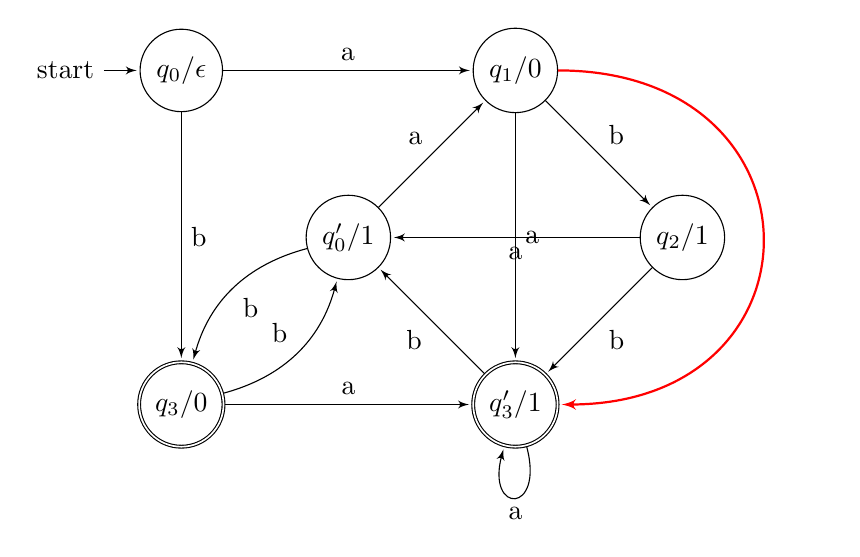
\begin{tikzpicture}[>=latex',shorten >=1pt,node distance=3cm,on grid,auto]
  \node[state,initial] (q0-e) {$q_0/\epsilon$};
  \node[state] (q0-1) [below right=of q0-e] {$q_0'/1$};
  \node[state] (q1-0) [above right=of q0-1] {$q_1/0$};
  \node[state] (q2-1) [below right=of q1-0] {$q_2/1$};
  \node[state,accepting] (q3-0) [below left=of q0-1] {$q_3/0$};
  \node[state,accepting] (q3-1) [below right=of q0-1] {$q_3'/1$};
  \path[->] (q0-e) edge node {a} (q1-0);
  \path[->] (q0-e) edge node {b} (q3-0);
  \path[->] (q0-1) edge node {a} (q1-0);
  \path[->] (q0-1) edge [bend right] node {b} (q3-0);
  \path[->] (q1-0) edge node {a} (q3-1);
  \path[->] (q1-0) edge node {b} (q2-1);
  \path[->] (q2-1) edge node {a} (q0-1);
  \path[->] (q2-1) edge node {b} (q3-1);
  \path[->] (q3-0) edge node {a} (q3-1);
  \path[->] (q3-0) edge [bend right] node {b} (q0-1);
  \path[->] (q3-1) edge [loop below] node {a} (q3-1);
  \path[->] (q3-1) edge node {b} (q0-1);
  \draw [->,thick,red] (q1-0) ..  controls  ($(q1-0)+(4cm,0)$) and
  ($(q3-1)+(4cm,0)$) ..  (q3-1);
\end{tikzpicture}

\end{document}
